\newpage
\section{Auswertung}
\subsection{PV-Generatorwirkungsgrad}
Die Messungen erfolgen bei 26°C um 12:37Uhr Ortszeit.
Nach Aufnahme der grafischen Kennlinie wird eine Auswertung vorgenommen, 
Der MPP wird mithilfe der Tangentensteigung abgeschätzt.
 
\begin{table}[!ht]
\centering
\caption{Messdaten von Strom und Spannung in Abhängigkeit von Bestrahlungsstärke}
\label{tab:230515_Messdaten_PVGenKennlinie}
\begin{tabular}{|l|l|l|l|l|l|l|l|}
\hline
\rowcolor[HTML]{76B900} 
                                            & $U_{Leer}$ in $V$ & $I_K$ in $A$ & $U_{MPP}$ in $V$ & $I_{MPP}$ in $A$ & E in $\frac{W}{m^2}$ & FF in \% & A in $m^2$ \\ \hline
\cellcolor[HTML]{cfe5a8}feststehnde Anlage  & 41,7              & 10           & 31,6             & 9,5            & 670,10                      & 0,72     & 0,36    \\ \hline
\cellcolor[HTML]{cfe5a8}nachgeführte Anlage & 41,6              & 9,7          & 32               & 9,37           & 650,00                      & 0,74     & 0,36     \\ \hline
\end{tabular}
\end{table}

\begin{equation}
\eta_{Gen}=\frac{P_{Gen}}{P_{Sonne}}=\frac{P_{MPP}}{E\cdot A_{Module}}
\label{eq:230514_Wirkungsgrad_Generator}
\end{equation}

\subsubsection{feststehende Anlage}
\begin{equation}
P_{MPP} = U_{MPP} \cdot I_{MPP}
\label{eq:230514_Leistung_im_MPP}
\end{equation}

Um den Wirkungsgrad des PV-Generators zu bestimmen muss zunächst die Leistung im MPP über Formel \autoref{eq:230514_Leistung_im_MPP} bestimmt werden:
\\
$$P_{MPP} = 31,6V \cdot 9,50A = 300,2W$$ 
\\
Die Leistung eingesetzt in Formel \autoref{eq:230514_Wirkungsgrad_Generator}:\\
$$\eta_{Gen,fest}=\frac{300,2W}{670\frac{W}{m^2}\cdot 8\cdot0,36 m^2}
=0,15557 \approx 15,56\%$$\\
Der Wirkungsgrad der feststehenden Anlage beträgt $15,56\%$.
\subsubsection{nachgeführte Anlage}
Um den Wirkungsgrad des PV-Generators zu bestimmen muss zunächst die Leistung im MPP über Formel \autoref{eq:230514_Leistung_im_MPP} bestimmt werden:
\\
$$P_{MPP} = 32V \cdot 9,037A = 289,18W$$ \\
Die Leistung eingesetzt in Formel \autoref{eq:230514_Wirkungsgrad_Generator}:\\
$$\eta_{Gen,nach}=\frac{289,18W}{650\frac{W}{m^2}\cdot 8\cdot 0,36 m^2}
=0,1544\approx 15,44\%$$\\
Der Wirkungsgrad der nachgeführten Anlage beträgt $15,44\%$.
\subsubsection{Bewertung der Ergebnisse}

Laut Datenblatt des SW-8046 beträgt der $P_{MPP}$ des Moduls bei $1000\frac{W}{m^2}$ bis zu $60Wp$.
Die Leistung eingesetzt in Formel \autoref{eq:230514_Wirkungsgrad_Generator}:\\
$$\eta_{Modul}=\frac{60W}{1000\frac{W}{m^2}\cdot 0,36 m^2}
=0,16\approx 16\%$$\\
Für monokristalline PV-Module aus dem Jahr 2008 ist ein Modul Wirkungsgrad von 14-18\% plausibel. Eine Wirkungsgradminderung von 3,75-7,5\% sind für einen Zeitraum von 15Jahren wahrscheinlich. Im Bezug auf die Wirkungsgrade sind die Module gut erhalten. Weitere Verlustquellen können die langen Kabel und geringfügige Beschädigungen der Solarzellen darstellen. Auffällig ist, dass der Wirkungsgrad der nachgeführten Anlage etwas geringer im Vergleich zur feststehenden Anlage ausfällt, obwohl der Ausrichtungswinkel günstiger ist. Diese Beobachtung ist auf die instabilen Wetterverhältnisse während den zwei Messungen zurückzuführen und die hieraus unterschiedliche Bestrahlungsstärke.
Die Wirkungsgrade für beide PV-Generatoren sind demnach naheliegend.


\subsection{Wechselrichter}
\subsubsection{Wirkungsgrad Kennlinie}
Laut Datenblatt hat der Wechselrichter Sunny Island 2012/2224 im Betrieb, ohne Last, einen Eigenverbrauch von 21W. 
In unserem Fall lag der Eigenverbauch ohne Last bei 29,7 W. 
Der Eigenverbrauch wird dabei nach Formel \autoref{eq:230509_Eigenverbrauch} aus der Leistung am LR im Leerlauf bestimmt. 
Der Eigenverbrauch des Wechselrichters hat seine Ursachen dabei größtenteils aus den Schaltvorgängen, der in ihm verbauten Halbleiter, und den Ohmschen Widerständen.

\begin{equation}
	P_{ Eigenverbrauch }= U_{ LR} \cdot I_{ LR }
\label{eq:230509_Eigenverbrauch}
\end{equation} 


\begin{table}[!ht]
    \caption{Messdaten der Ströme, Spannungn und Leistungen }
	\centering
	\renewcommand{\arraystretch}{2}
\begin{tabularx}{\linewidth}{|r|X|X|X|X|X|X|X|X|X|X|X|}
\hline
\rowcolor[HTML]{76B900} 
{\color[HTML]{000000} Aufgabe}          & {\color[HTML]{000000} $P_{Sonne}$} & {\color[HTML]{000000} $U_{Gen}$} & {\color[HTML]{000000} $I_{Gen}$} & {\color[HTML]{000000} $U_{LR}$} & {\color[HTML]{000000} $I_{LR}$} & {\color[HTML]{000000} $I_{Batt}$} & {\color[HTML]{000000} $I_{WR}$} & {\color[HTML]{000000} $P_{AC}$} & {\color[HTML]{000000} $U_{AC}$} & {\color[HTML]{000000} $I_{AC}$} & {\color[HTML]{000000} f} \\ \hline
\rowcolor[HTML]{FFFFFF} 
\cellcolor[HTML]{CFE5A8}${WR}_{allein}$      & 690                             & 39,3                          & 0,84                          & 25,4                         & 1,17                         & 0,15                           & 0,97                         & 12                           & 229,83                       & 0                            & 50Hz                       \\ \hline
\rowcolor[HTML]{FFFFFF} 
\cellcolor[HTML]{CFE5A8}$Staub_{1}$        & 550                             & 33,6                          & 7,84                          & 24,5                         & 8,9                          & -10,5                          & 21,9                         & 510                          & 228,5                        & 3,04                         & 55Hz\\ \hline
\rowcolor[HTML]{FFFFFF} 
\cellcolor[HTML]{CFE5A8}$Staub_{2}$        & 460                             & 32,2                          & 12,49                         & 23,3                         & 15,6                         & -27,2                          & 43,4                         & 942                          & 227,47                       & 4,33                         & 50Hz\\ \hline
\rowcolor[HTML]{FFFFFF} 
\cellcolor[HTML]{CFE5A8}$Staub_{3}$        & 471                             & 36,8                          & 7,66                          & 23,2                         & 10,94                        & -46,2                          & 57,3                         & 1208                         & 226,98                       & 5,05                         & 50Hz\\ \hline
\rowcolor[HTML]{FFFFFF} 
\cellcolor[HTML]{CFE5A8}S-Bahn Heizung & 601                             & 34,8                          & 16,15                         & 23,2                         & 20,51                        & -33,7                          & 55,7                         & 1186                         & 227,4                        & 5                            & 50Hz                    \\ \hline
\end{tabularx}
	\label{tab:230512_Messtabelle}
\end{table}

Der Wirkungsgrad des Wechselrichters berechnet sich nach folgender Formel:
%
\begin{equation}
	\eta_{ WR} = \frac{ P_{AC} }{ P_{WR,Ein} }
	\label{eq:230509_Wirkungsgrad}
\end{equation}
%
%
\begin{figure}[!ht]
		\centering
		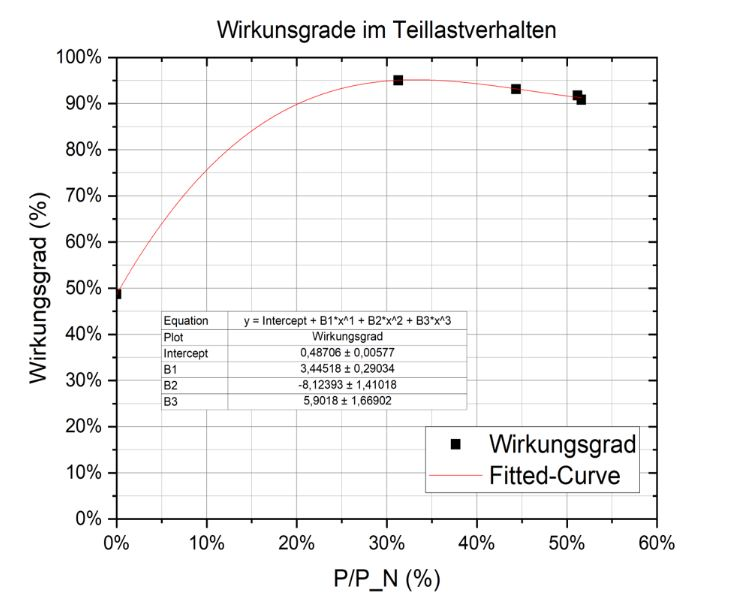
\includegraphics[width=0.7\textwidth]{Abbildungen/Kennlinie wr}
		\caption{Wirkungsgradkennlinie des Wechselrichters in Abhängigkeit der Auslastung}
		\label{fig:230512_WRkennlinie}
\end{figure}
%
\begin{table}[]
 \caption{Wirkungsgrad und Leistungsbeiwert}
	\centering
\begin{tabular}{|r|r|r|r|r|r|}
\hline
\rowcolor[HTML]{76B900} 
Aufgabe                                  & $WR_{allein}$ & $Staubsauger_1$ & $Staubsauger_2$ & $Staubsauger_3$ & S-Bahn Heizung \\ \hline
\cellcolor[HTML]{cfe5a8}Wirkungsgrad\_WR & 49\%       & 95\%     & 93\%     & 91\%     & 92\%            \\ \hline
\cellcolor[HTML]{cfe5a8}cos(phi)         & 0,00       & 0,73     & 0,96     & 1,05     & 1,04            \\ \hline
\end{tabular}
\end{table}
Dabei ist in \autoref{fig:230512_WRkennlinie} zu erkennen, dass der Wirkungsgrad des Wechselrichters sich nicht linear verhält. Zunächst ist sehr niedrig und nähert sich dann einem Maximum an. Anschließend fällt der Wirkungsgrad wieder leicht ab, was an den steigenden Ohmschenverlusten liegt, die bei immer höher werdenen Strömen immer größer werden. Der maximale Wirkungsgrad liegt bei uns sogar bei 95 Prozent (\autoref{fig:230512_WRkennlinie}). Dies ist sogar 2 Prozent über dem Wirkungsgrad den der Hersteller angibt. Die ermittelte Kurve für den Wirkungsgrad ist dabei gut mit der Theorie zu vereinbaren. Des Weiteren ist zu erkennen, dass dieser Wechselrichter bereits ab 30 \% der Nennleistung sehr hohe Wirkungsgrade beseitzt, was ihn besonders gut macht für Standorte, die häufig Teilleistung liefern.
\subsubsection{Frequenz- und Spannungsstabilität}
Wie in unseren Messwerten zu sehen liegt die Spannung zwischen 226V und 230V. 
Die Spannung nimmt dabei mit steigender Leistung ab. 
Diese Werte passen auch sehr gut mit den Datenblattwert von 230 Volt zusammen. 
Die Frequenz bleibt dabei konstant bei 50 Hertz, wie man auf den Osziloskopbildern erkennen kann. 
Jedoch ist auch zu erkennen, dass der Sinus nur im Leerlauf und beim Anschließen der Straßenbahnheizung ohne Oberschwingungen daherkommt. 
Dies liegt daran, das hier ausschließlich Wirkleistung benötigt wird. 
Beim Anschließen des Staubsaugers erkennt man in \autoref{fig:oszi} die Oberschwingungen die entstehen. 
Dies liegt daran, dass der Staubsauer auch Blindleistung benötigt.
%
% \begin{figure}[!ht]
% 		\centering
% 		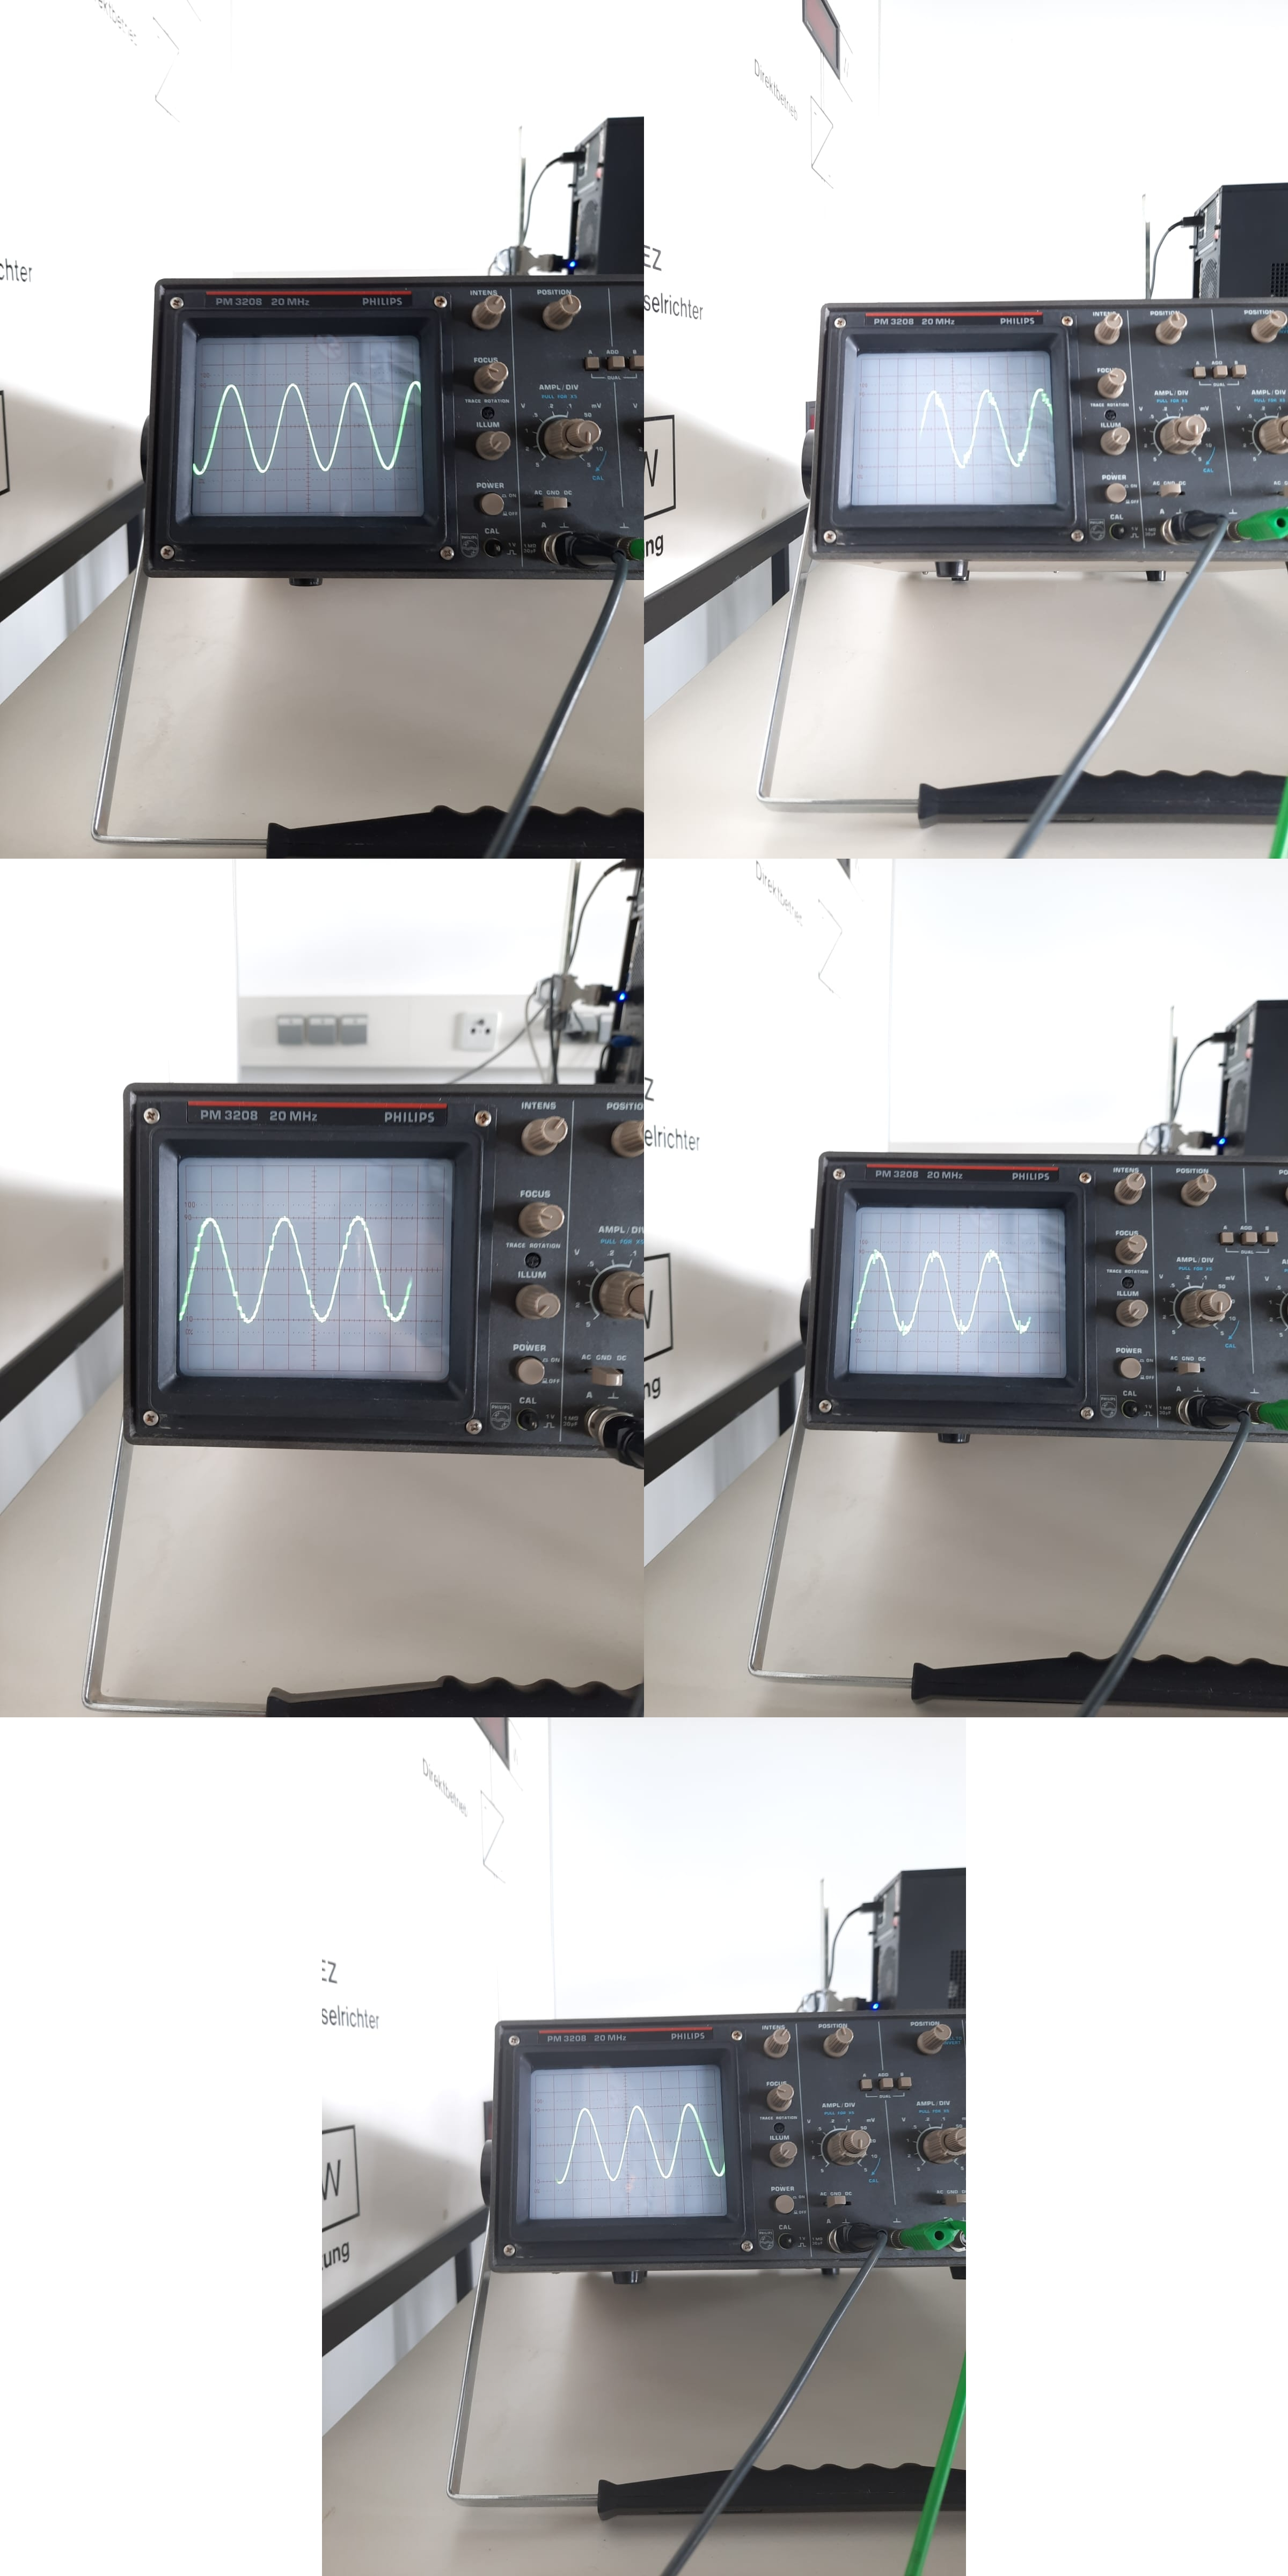
\includegraphics[width=0.5\textwidth]{Abbildungen/MergedImages}
% 		\caption{Von links nach rechts sieht man hier die Osziloskopbilder des Versuchs zuerst im Leerlauf, dann mit dem Staubsauger von Stufe 1-3 und im letzten Bild wurde die Straßenbahnheizung angeschlossen.}
% 		\label{fig:oszi}
% \end{figure}
%

\begin{figure}[H]
	\centering
	\begin{subfigure}[c]{0.19\textwidth}
		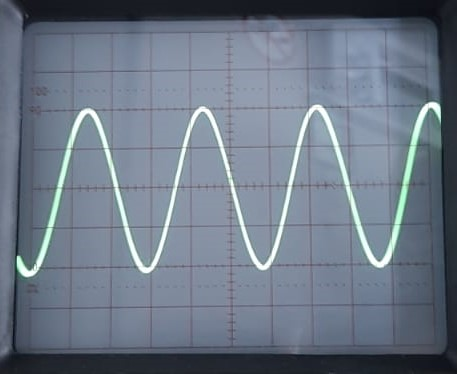
\includegraphics[width=\textwidth]{Abbildungen/Oszi_Leerlauf.jpg}
		\caption{Leerlauf}
	\end{subfigure}
	\begin{subfigure}[c]{0.19\textwidth}
		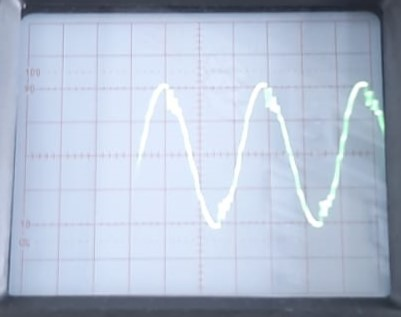
\includegraphics[width=\textwidth]{Abbildungen/Oszi_Staub_1.jpg}
		\caption{Staub 1}
	\end{subfigure}
	\begin{subfigure}[c]{0.19\textwidth}
		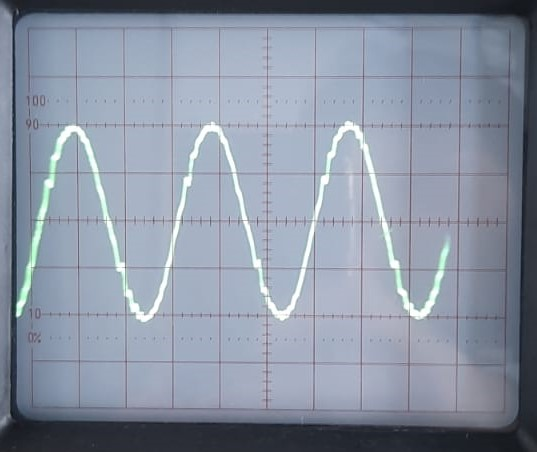
\includegraphics[width=\textwidth]{Abbildungen/Oszi_Staub_2.jpg}
		\caption{Staub 2}
	\end{subfigure}
	\begin{subfigure}[c]{0.19\textwidth}
		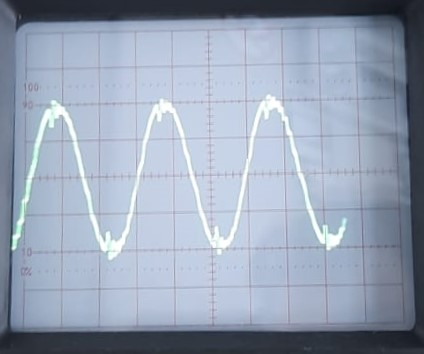
\includegraphics[width=\textwidth]{Abbildungen/Oszi_Staub_3.jpg}
		\caption{Staub 3}
	\end{subfigure}
	\begin{subfigure}[c]{0.19\textwidth}
		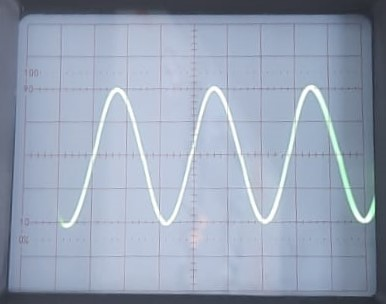
\includegraphics[width=\textwidth]{Abbildungen/Oszi_S-Bahn_Heiz.jpg}
		\caption{S-Bahn Heizung}
	\end{subfigure}
	\caption{Osziloskopbilder bei verschiedenen Belastungen}
	\label{fig:oszi}
\end{figure}


\subsubsection{Leistungsbeiwert}
Der Leistungsbeiwert $ \cos(\phi) $ berechnet sich nach \autoref{eq:230509_Cos(phi)}:
%
\begin{equation}
	\cos(\phi)=\frac{ P_{ AC,Wirk } }{  I_{ AC } \cdot U_{AC }}
	\label{eq:230509_Cos(phi)}
\end{equation}
%
Dabei ist in der Tabelle zu sehen, dass bei immer größerer Leistung beim Staubsauger der Leistungsbeiwet sich immer näher an 1 annähert (\autoref{tab:150523_Messtabelle}), was bedeutet, dass fast nur Wirkleistung benötigt wird. 
Leider ist es nicht möglich den Leistungsbeiwert anhand unserer Oszilosgramme zu bestimmen. 
Dies liegt daran, dass es nicht möglich war ein stehendes Bild zu erzeugen, anhand dessen es möglich wäre eine Aussage über den Phasenversatz zu machen. 
In der Theorie sollte mit steigendem Blindleistungsbedarf ein immer größer Phasenversatz zu sehen sein.

\subsection{Leistungsbilanz}
\subsubsection{Leistungsbilanz}
\begin{table}[!ht]
\centering
\caption{Leistungsbilanz}
\renewcommand{\arraystretch}{1.5}
\begin{tabularx}{\textwidth}{|X|X|X|X|X|X|X|X|}
\hline
\rowcolor[HTML]{76B900} 
$P_{Sonne}$ & $P_{Gen_{DC}}$ & $P_{LR}$ & $P_{Bat}$ & $P_{WR}$ & $P_{AC}$ & $P_{Verluste}$ & Verluste \\ \hline
690$\frac{W}{m^2}$                              &  33,01$W$                & 29,72$W$          &   -3,81$W$            &   24,64$W$          & 12$W$              & 17,20$W$                  & 59\%    \\ \hline
550$\frac{W}{m^2}$                              & 263,42$W$               & 218,05$W$          &  257,25$W$           &  536,55$W$          & 510$W$             & 10,67$W$                  & 2,05\%    \\ \hline
460$\frac{W}{m^2}$                              & 402,18$W$               & 363,48$W$          &  633,76$W$           & 1011,22$W$         & 942$W$             & 93,94$W$                  & 9,07\%    \\ \hline
471$\frac{W}{m^2}$                              & 281,89$W$               & 253,81$W$         & 1071,84$W$          & 1329,36$W$         & 1208$W$            & 145,73$W$                 & 10,8\%    \\ \hline
601$\frac{W}{m^2}$                              & 562,02$W$                & 475,83$W$         &  781,84$W$           & 1292,24$W$         & 1186$W$            & 157,86$W$                  & 11,75\%    \\ \hline
\end{tabularx}
\label{tab:230514_Leistungsbilanz}
\end{table}



\subsubsection{Verlustquellen}
\begin{figure}[!ht]
		\centering
		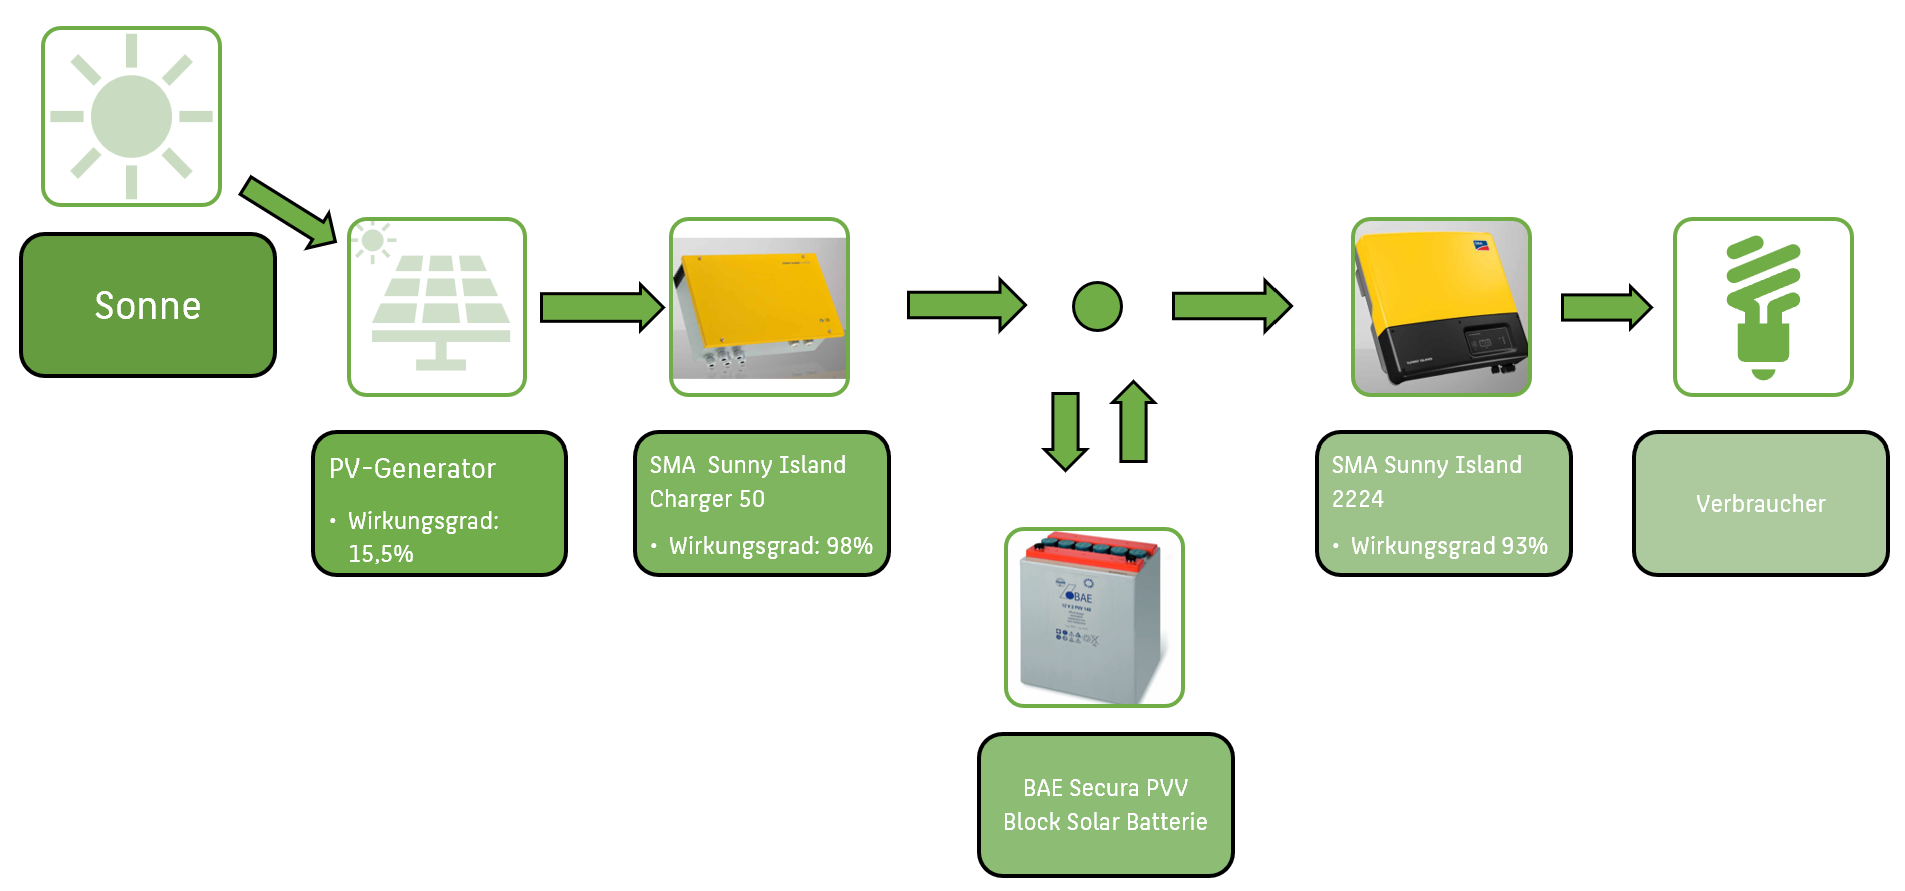
\includegraphics[width=\linewidth]{Abbildungen/Leistungsbilanz.png}
		\caption{Leistungsbilanz der Anlage}
		\label{fig:230512_Leistungsbilanz}
\end{figure}

\autoref{fig:230512_Leistungsbilanz} stellt schematisch den Anlagenaufbau und Leistungsfluss dar. Hierbei ist der erste Verlustfaktor der Anlagenwirkungsgrad da nicht 100\% der Sonnenenergie in Leistung umgewandelt werden kann. Der Wirkungsgrad des verwendeten Ladereglers liegt bei 98\%, womit es zu geringfügigen Verlusten kommt. Je nachdem ob es einen Leistungsüberschuss oder ein Leistungsdefizit gibt, stellt die Batterie Strom zur Verfügung. Die Selbstentladung von 2\% pro Monat der Batterie kann in diesem Fall vernachlässigt werden, da im betrachteten Fall die Messdauer sehr kurz ist. Der Wechselrichter besitzt einen Wirkungsgrad von 93\%. Im Wechselrichter kommt es zu den höchsten Umwandlungsverlusten bei der Umwandlung von DC in AC Spannung.
Die Länge der Kabel stellen eine weitere Verlustquellen dar.


\subsubsection{Vor-und Nachteile Direktbetrieb einer PV-Anlage}
Vorteilhaft am Direktbetrieb einer PV-Anlage sind vorallem die günstigen Kosten durch das Wegfallen von Batterie, Laderegler und Wechselrichter.


